\begin{frame}[fragile,t]
\frametitle{Übersicht}
\tableofcontents
\end{frame}
\section{Tabellen, Listen, Boxen}
\subsection{Tabellen}

\begin{frame}[fragile]
\frametitle{tabular}
\begin{itemize}[<+->]
  \item Tabellen werden mit der \texttt{tabular}-Umgebung erzeugt. Die Syntax ist 
    \begin{lstlisting}[style=Latex]
\begin{tabular}[Position]{<Spaltenformatierung>}
<Inhalt>
\end{tabular}
\end{lstlisting}\vspace{-20pt}
  \item gültige \texttt{<Position>} Parameter sind
  \begin{itemize}
    \item \texttt{l,r,c}: linksbündige / rechtsbündige / zentrierte Spalte
  \end{itemize}
  \item mit einem \lstinline[style=Latex]+&+ nächste Spalte
  \item mit einem \lstinline[style=Latex]+\\+ nächste Zeile
  \item horizontale Linien werden erzeugt durch:
  \begin{itemize}
    \item \lstinline[style=Latex]|\hline| Linie über die gesamte Breite
  \end{itemize}
\end{itemize}
\end{frame}


\begin{frame}[fragile,t]
\frametitle{Beispiel}
\begin{lstlisting}[style=Latex]
\begin{tabular}{r|c||l|}
rechts & zentriert & links \\ \hline
wieder & alles & normal
\end{tabular}
\end{lstlisting}
\pause\vspace{-20pt}
\result{
\begin{tabular}{r|c||l|}
rechts & zentriert & links \\ \hline
wieder & alles & normal\\
\end{tabular}}
\end{frame}

\begin{frame}[fragile,t]
\frametitle{Noch zu Tabellen}
Tabellen lassen sich jedoch noch leichter durch Onlinetools wie
\begin{center}
\url{http://www.tablesgenerator.com/}
\end{center}
erstellen.

\begin{figure}[htp]
\centering
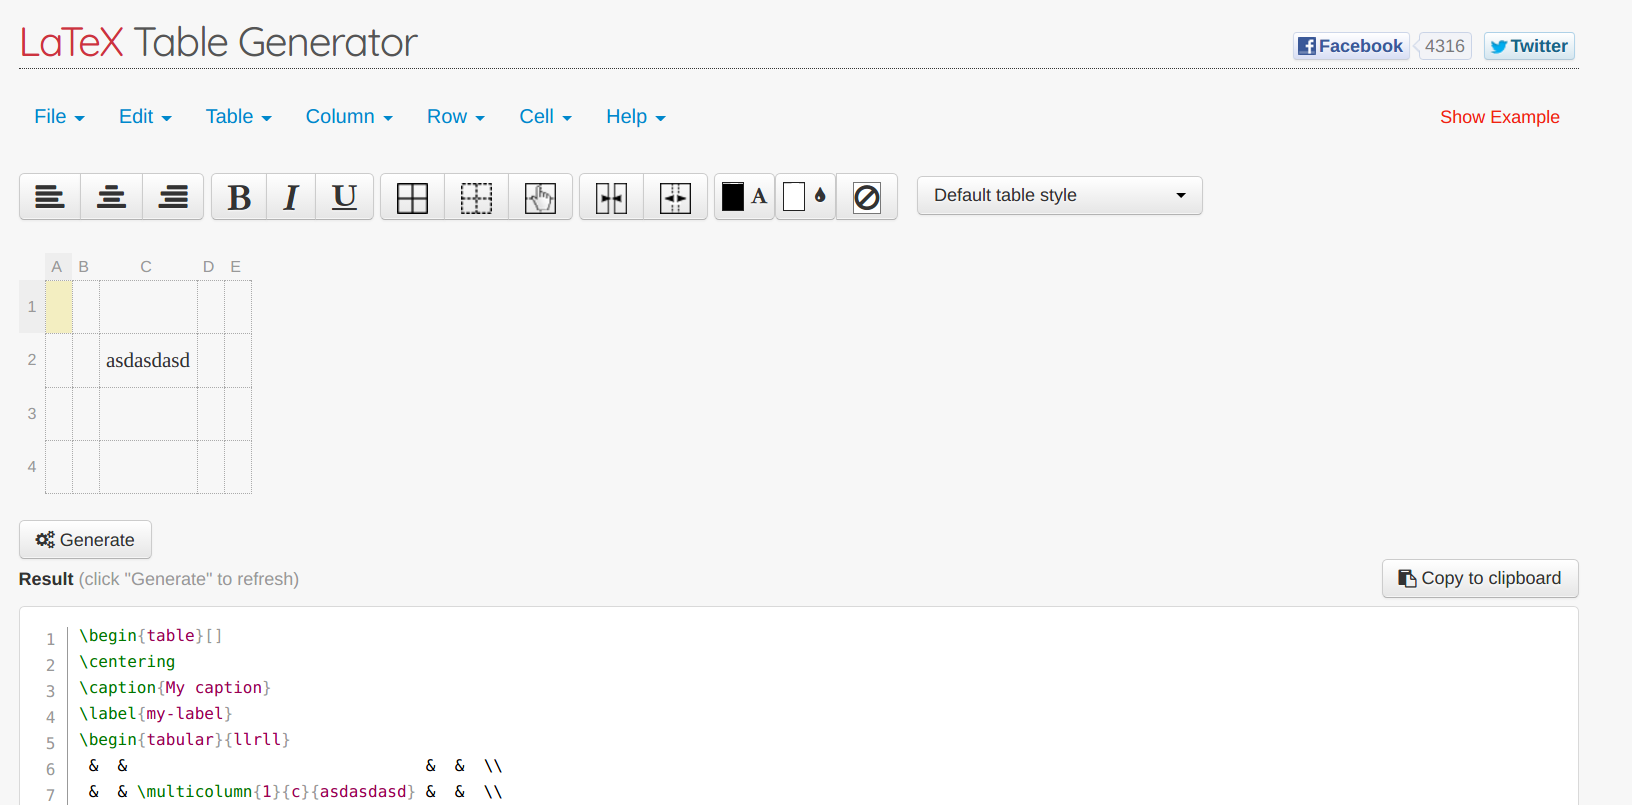
\includegraphics[scale=0.18]{images/onlinetable.png}
\end{figure}
\end{frame}



\subsection{Listen}

\begin{frame}[fragile]
\frametitle{Listen}
\begin{itemize}[<+->]
  \item Listen werden durch die \texttt{itemize}-Umgebung erzeugt.
  \item durch \lstinline[style=Latex]+\item+ wird ein Aufzählungspunkt erzeugt. Als optionaler Parameter kann das Aufzählungszeichen angegeben werden.
\end{itemize}
\end{frame}

\begin{frame}[fragile,t]
\frametitle{Beispiel 1}\vspace{-10pt}
\begin{lstlisting}[style=Latex]
\begin{itemize}
  \item Punkt 1
  \begin{itemize}
    \item Unterpunkt 1
    \item Unterpunkt 2
  \end{itemize}
  \item[*] Punkt 2
  \item Punkt 3
\end{itemize}
\end{lstlisting}
\pause\vspace{-25pt}
\result{\vspace{-10pt}
\begin{itemize}
  \item Punkt 1
  \begin{itemize}
    \item Unterpunkt 1
    \item Unterpunkt 2
  \end{itemize}
  \item[*] Punkt 2
  \item Punkt 3
\end{itemize}\vspace{-10pt}}
\end{frame}
\begin{frame}[fragile]
\frametitle{Listen}
Aufzählungen werden analog durch \texttt{enumerate} erzeugt.
\end{frame}
\begin{frame}[fragile,t]
\frametitle{Beispiel 2}\vspace{-10pt}
\begin{lstlisting}[style=Latex]
\begin{enumerate}
  \item Punkt 1
  \begin{enumerate}
    \item Unterpunkt 1
    \item Unterpunkt 2
  \end{enumerate}
  \item Punkt 2
  \item Punkt 3
\end{enumerate}
\end{lstlisting} 
\pause\vspace{-25pt}
\result{\vspace{-10pt}
\begin{enumerate}
  \item Punkt 1
  \begin{enumerate}
    \item Unterpunkt 1
    \item Unterpunkt 2
  \end{enumerate}
  \item Punkt 2
  \item Punkt 3
\end{enumerate}\vspace{-10pt}}
\end{frame}
\begin{frame}[fragile]
\frametitle{Listen}
Mithilfe des Pakets \texttt{enumerate} können die Aufzählungszeichen leicht geändert werden.
\end{frame}
\begin{frame}[fragile,t]
\frametitle{Beispiel 3}\vspace{-10pt}
\begin{lstlisting}[style=Latex]
\begin{enumerate}[(i)]
  \item Punkt 1
  \begin{enumerate}[a)]
    \item Unterpunkt 1
    \item Unterpunkt 2
  \end{enumerate}
  \item Punkt 2
  \item Punkt 3
\end{enumerate}
\end{lstlisting} 
\pause\vspace{-25pt}
\result{\vspace{-10pt}
\begin{enumerate}[(i)]
  \item Punkt 1
  \begin{enumerate}[a)]
    \item Unterpunkt 1
    \item Unterpunkt 2
  \end{enumerate}
  \item Punkt 2
  \item Punkt 3
\end{enumerate}\vspace{-10pt}}
\end{frame}
\begin{frame}[fragile]
\frametitle{Listen}
 Aufzählungen mit Namen für jeden Punkt werden durch \texttt{description} erzeugt.
\begin{itemize}[<+->]
  \item das Aussehen dieser Listen variiert je nach Dokumentenklasse!
  \item durch Ändern der Variablen \lstinline[style=Latex]+\labelitemi+, \lstinline[style=Latex]+\labelitemii+, etc können die Aufzählungssymbole global geändert werden.
\end{itemize}
\end{frame}
\begin{frame}[fragile]
\frametitle{Beispiel 4}
\begin{lstlisting}[style=Latex]
\begin{description}
  \item[Label 1] Punkt 1
  \item[toller Name] Punkt 2
  \item[Bla] Punkt 3
\end{description}
\end{lstlisting} \vspace{-20pt}
\pause\result{
\begin{description}
  \item[Label 1] Punkt 1
  \item[toller Name] Punkt 2
  \item[Bla] Punkt 3
\end{description}}
\end{frame}
\begin{comment}
\subsection{Tabulatoren}


\begin{frame}[fragile]
\frametitle{tabulatoren}
\begin{itemize}[<+->]
  \item Tabulatoren können in der \texttt{tabbing}-Umgebung verwendet werden.
  \item Steuerzeichen sind:
  \begin{itemize}
    \item \lstinline[style=Latex]+\=+ neuer Tabulator
    \item \lstinline[style=Latex]+\\+ neue Zeile
    \item \lstinline[style=Latex]+\>+ nächster Tabulator
    \item \lstinline[style=Latex]+\<+ ein Tabulator zurück
    \item \lstinline[style=Latex]|\+| wie \lstinline[style=Latex]+\>+ nur über Zeilengrenzen hinweg
    \item \lstinline[style=Latex]+\-+ wie \lstinline[style=Latex]+\<+ nur über Zeilengrenzen hinweg
    \item \lstinline[style=Latex]+\'+ Tabsprung und zentriert den vorherigen Tab
    \item \lstinline[style=Latex]+\kill+ blendet die letzte Zeile aus (für Musterzeile)
  \end{itemize}
\end{itemize}
\end{frame}

\begin{frame}[fragile,t]
\frametitle{Beispiel}\vspace{-10pt}
\begin{lstlisting}[style=Latex]
\begin{tabbing}
 Breite 1 \= Breite 2 \= B3 \= Breite 4 \kill
 T1 \> T2 \> \> Tablulator 3 \+ \\
 A1 \> A2 \> A3 \\
 Text \= vieeeeeel zu lang \> Text 2 \\
 \> in neuen Tab \\
 \< wieder an Anfangstab 
\end{tabbing}
\end{lstlisting} 
\pause\vspace{-20pt}
\result{\vspace{-15pt}
\begin{tabbing}
 Breite 1 \= Breite 2 \= B3 \= Breite 4 \kill
 T1 \> T2 \> \> Tablulator 3 \+ \\
 A1 \> A2 \> A3 \\
 Text \= vieeeeeel zu lang \> Text 2 \\
 \> in neuen Tab \\
 \< wieder an Anfangstab 
\end{tabbing}\vspace{-15pt}}
\end{frame}
\end{comment}


\begin{comment}
\begin{frame}[fragile]
\frametitle{Boxen}
\begin{itemize}[<+->]
  \item In \LaTeX\, dienen Boxen dazu, den Inhalt als ein einzelnes Objekt zu betrachten. Dies hat mehrere Vorteile:
  \begin{itemize}
    \item die Box kann verschoben werden
    \item der Box können Grenzen angegeben werden
    \item sie kann eingerahmt werden
  \end{itemize}
  \item Syntax: \lstinline[style=Latex]+\makebox[<Breite>][<Pos>]{<Inhalt>}+
  \item als Position sind gültig:
  \begin{itemize}
    \item leer: zentriert
    \item \texttt{l}: linksbündig
    \item \texttt{r}: rechtsbündig
    \item \texttt{s}: gestreckt
  \end{itemize}
  \item automatische Breite: \lstinline[style=Latex]+\mbox+
  \item umrahmte Boxen: \lstinline[style=Latex]+\framebox+ bzw. \lstinline[style=Latex]+\fbox+.
\end{itemize}
\end{frame}

\begin{frame}[fragile]
\frametitle{raisebox}
\begin{itemize}[<+->]
  \item Boxen können verschoben werden mit
    \lstinline[style=Latex]+\raisebox{<Lift>}[<oben>][<unten>]{<Inhalt>}+
  \item dabei bedeuten
  \begin{itemize}
    \item \texttt{<Lift>}: soviel wird die Box angehoben
    \item \texttt{<oben>}: Abstand zur oberen Linie
    \item \texttt{<unten>}: Abstand zur unteren Linie
  \end{itemize}
\end{itemize}
\end{frame}
\end{comment}

\subsection{Minipage}

\begin{frame}[fragile]
\frametitle{minipage}
\begin{itemize}[<+->]
  \item Syntax: 
  \begin{lstlisting}[style=Latex]
\begin{minipage}[<Pos>]{<Breite>}
<Inhalt>
\end{minipage}
\end{lstlisting}\vspace{-20pt}
  \item \texttt{<Breite>} können in den bekannten Einheiten angegeben werden
  \begin{itemize}
    \item beachte die Verwendung von Konstanten wie \lstinline[style=Latex]+\textwidth+!
  \end{itemize}
  \item \texttt{<Pos>}: welche Zeile soll mit der aktuellen abschließen:
  \begin{itemize}
    \item \texttt{t}: oberste Zeile der Box
    \item \texttt{b}: unterste Zeile der Box
    \item nichts: Box wird zentriert
  \end{itemize}
%  \item \texttt{<iPos>}: Textanordnung innerhalb der Box:
%  \begin{itemize}
%    \item \texttt{t}: Text schließt oben ab
%    \item \texttt{b}: Text schließt unten ab
%    \item \texttt{c}: Text wird mittig zentriert
%    \item ohne: Text wird über die gesamge Höhe gestreckt
%  \end{itemize}
\end{itemize}
\end{frame}



\begin{frame}[fragile,t]
\frametitle{Beispiel}
\begin{lstlisting}[style=Latex]
\begin{minipage}{.49\textwidth}
Linke Minipage
\end{minipage}
\begin{minipage}{.49\textwidth}
Rechte Minipage
\end{minipage}
\end{lstlisting}\pause
\result{
\begin{minipage}{.49\textwidth}
Linke Minipage
\end{minipage}
\begin{minipage}{.49\textwidth}
Rechte Minipage
\end{minipage}}

\end{frame}
